\section{Syntax-Semantic Completeness}\label{sec:complete}

Finally, we prove that our semantics, namely that of Parametric Linear Programs, is fully axiomatized by the constructed SMT \textbf{GLP}. This section is divided into three parts:

\begin{itemize}
	\item Proving Soundness: a check that every
	      generator is correctly interpreted and all our axioms
	      are sound with respect to the semantics.
	\item Definability: that every semantic object, i.e.\ a
	      \textit{Parametric Linear Program}, has a standard normal form, and
	      that this normal form is always the interpretation of some diagram.
	\item Completeness: through the epigraph form, any two identical PLPs
	      can be reduced to the same polyhedron, which in turn makes their diagrams equal.
\end{itemize}

Together, these three properties establish that the semantics is fully axiomatised.

\begin{lemma}[Soundness]
	If $s = t$ in $\mathrm{FreeP}_{\mathbf{GLP}}$, then $[s] = [t]$
	in $\mathbf{PolyFun}$.
\end{lemma}

\begin{proof}
	All axioms inherited from $\mathbf{GPA}$ are already sound by the
	results of the previous section. It suffices to verify that the new
	axioms involving the LP generator preserve the semantics, which
	follows by direct computation:
	\begin{figure}[H]
		\centering
		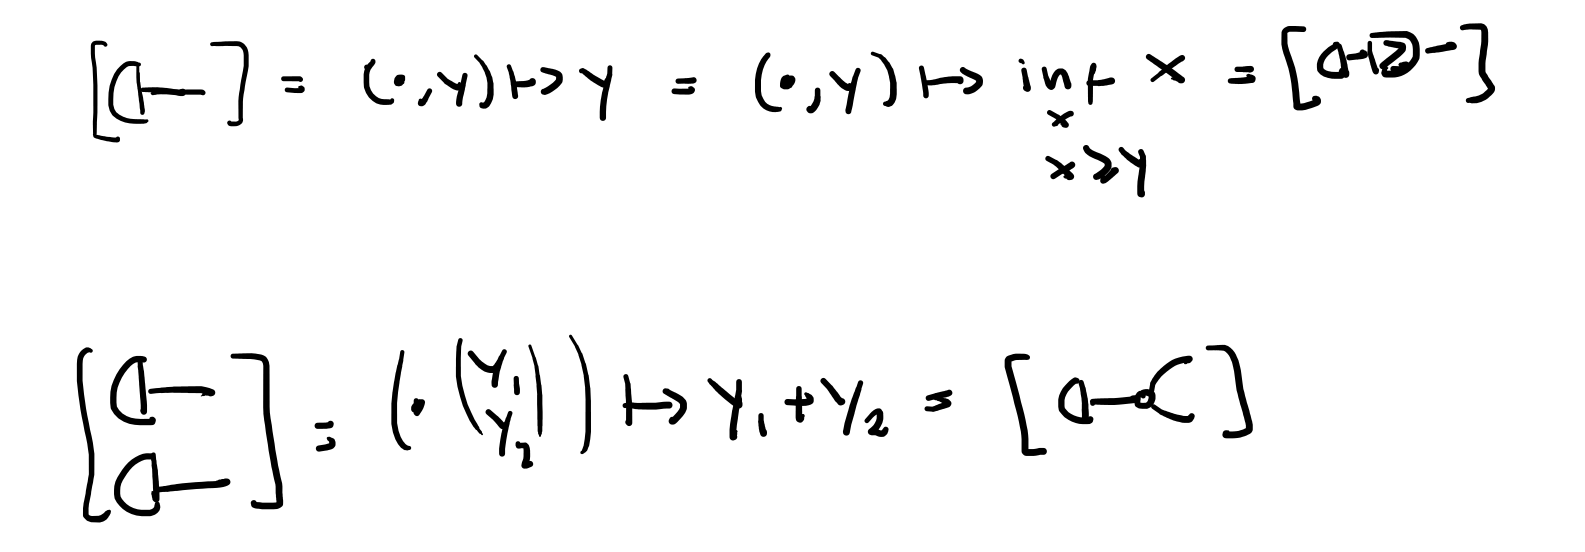
\includegraphics[width=0.75\linewidth]{../images/GLP/Soundness.png}
	\end{figure}
\end{proof}

\begin{lemma}[Definability / Expressivity]
	For every $f : m \to n$ in $\mathbf{LPRel}$ there exists a
	$\Sigma$-term $s : m \to n$ in
	$\mathrm{Hom}_{\mathrm{FreeP}_{\mathbf{GLP}}}(m,n)$
	such that $[s] = f$.
\end{lemma}

\begin{proof}
	Since every RHS PLP admits a standard form,
    it suffices to show that every piecewise affine
	convex function is expressible in $\mathbf{GLP}$. For an arbitrary
	such function $f(y) = \inf_x c^\top x$, where $A x + b \ge B y$
    the following diagram provides the required syntactic representative:
    \begin{figure}[H]
        \centering
        \begin{tikzpicture}[axpic]

                  % Left bracket
            \node[scale=1.5] at (0.25,1.0) {$\llbracket$};

                  % Main diagram
                  \begin{scope}[shift={(0.000,1.000)}]
                    \pic (g1) at (0.500,0.500) {linear};

                    \begin{scope}[shift={(1.250,0.000)}]
                      \pic[val=c^\top] (g2) at (0.500,0.500) {coscalar};
                    \end{scope}

                    \draw (g1-out-0) to[out=0,in=180] (g2-in-0);

                    \begin{scope}[shift={(2.500,0.000)}]
                      \pic[val=A] (g3) at (0.500,0.500) {matrix};
                    \end{scope}

                    \draw (g2-out-0) to[out=0,in=180] (g3-in-0);
                  \end{scope}

                  \begin{scope}[shift={(1.250,0.000)}]
                    \pic (g4) at (0.500,0.500) {affine};
                  \end{scope}

                  \coordinate (a5) at (3.500,0 |- g4-out-0);
                  \draw (g4-out-0) -- (a5);

                  \begin{scope}[shift={(3.750,0.500)}]
                    \pic (g6) at (0.500,0.500) {multiplication};
                  \end{scope}

                  \draw (g3-out-0) to[out=0,in=180] (g6-in-0);
                  \draw (a5)       to[out=0,in=180] (g6-in-1);

                  \begin{scope}[shift={(5.000,0.500)}]
                    \pic (g7) at (0.500,0.500) {ge};
                  \end{scope}

                  \draw (g6-out-0) to[out=0,in=180] (g7-in-0);

                  \begin{scope}[shift={(6.250,0.500)}]
                    \pic[val=B] (g8) at (0.500,0.500) {comatrix};
                  \end{scope}

                  \draw (g7-out-0) to[out=0,in=180] (g8-in-0);

                  \node[scale=1.5, anchor=west] at ($(g8-out-0)-(0.06,0)$) {$\rrbracket$};
                  % Right bracket and meaning, anchored relative to the diagram
                  \node[anchor=west] at ($(g8-out-0)+(0.25,0)$)
                    {$
                      = y \mapsto \inf_x c^\top x
                      \ \text{s.t.}\ 
                      Ax + b \ge By$};

        \end{tikzpicture}
    \end{figure}
\end{proof}

The final result is the completeness theorem for
$\mathbf{GLP}$. The proof brings together the main tools developed
throughout: the epigraph form (Corollary~\ref{cor:epigraph form}), the
shared epigraph property (Proposition~\ref{prop:equalepi}), the
completeness of $\mathbf{GPA}$, and the FME-based normal form. It
relies on the completeness of the $\mathbf{GPA}$
polyhedra case (Theorem~\ref{thm:gpapresent}); given
that result, the argument below goes through.

\begin{lemma}[Completeness]
	If $[c] = [d]$ in $\mathbf{PolyFun}$, then $c = d$ in
	$\mathrm{FreeP}_{\mathbf{GLP}}$.
\end{lemma}

\begin{proof}
	Let $v_1 = [c]$ and $v_2 = [d]$. By assumption $v_1 = v_2$, so
	Proposition~\ref{prop:equalepi} gives
	$\mathrm{epi}(v_1) = \mathrm{epi}(v_2) =: E$.

	By Corollary~\ref{cor:epigraph form}, both $c$ and $d$ admit
	epigraph forms $c = \mushroom ; c^*$ and $d = \mushroom ; d^*$
	with $[c^*] = [d^*] = E$ in $\mathbf{PolyRel}$:
	\begin{figure}[H]
		\centering
		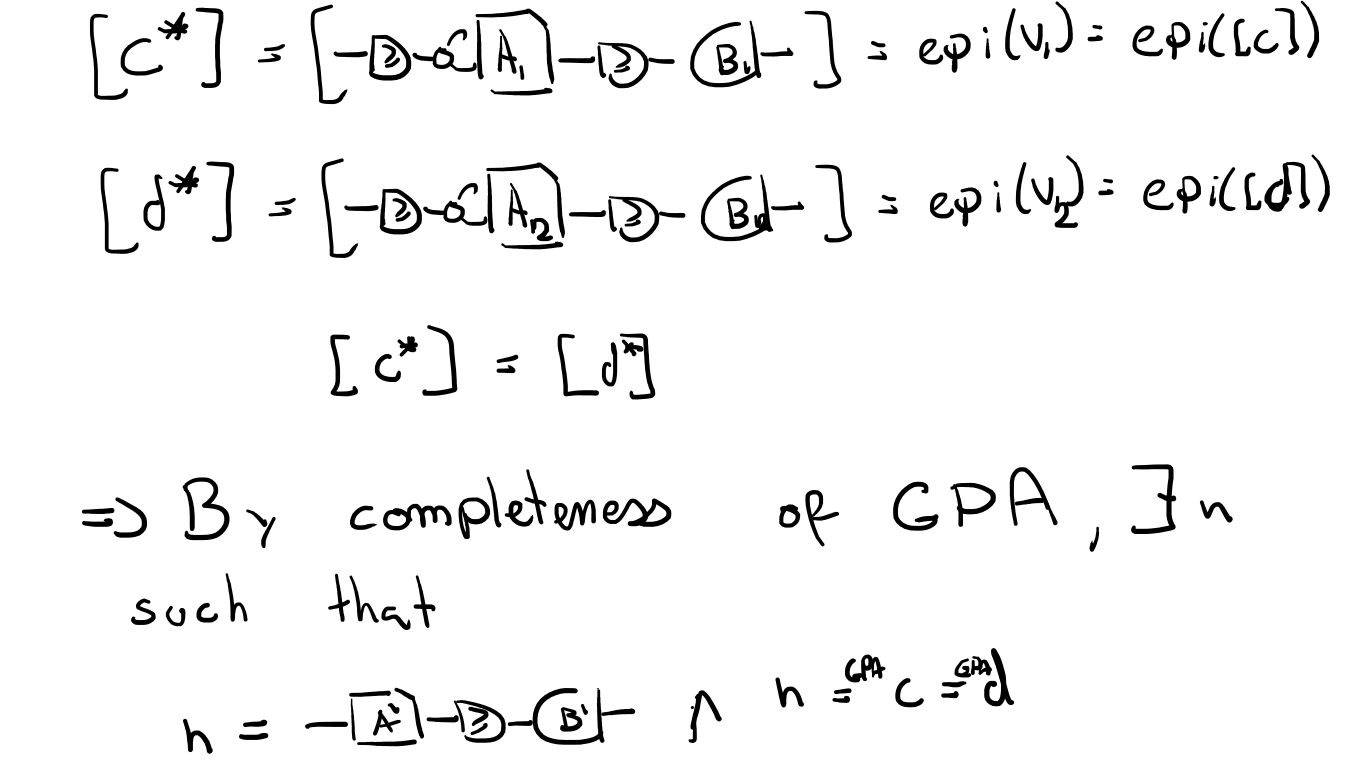
\includegraphics[width=0.75\linewidth]{../images/GLP/proofCompleteness1.png}
	\end{figure}
	Since $[c^*] = [d^*]$ in $\mathbf{PolyRel}$, completeness of
	$\mathbf{GPA}$ gives $c^* = d^*$ in
	$\mathrm{FreeP}_{\mathbf{GPA}}$. Therefore,
	\[
		c = \mushroom ; c^* = \mushroom ; d^* = d,
	\]
	as witnessed diagrammatically by:
	\begin{figure}[H]
		\centering
		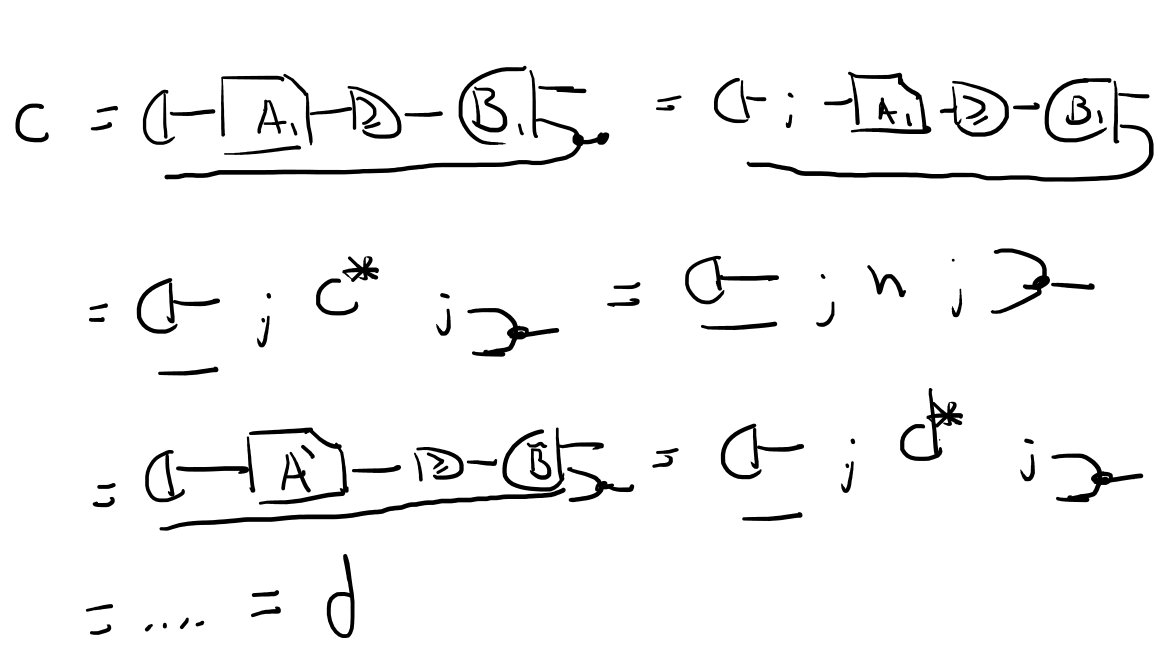
\includegraphics[width=0.75\linewidth]{../images/GLP/proofCompleteness4.png}
	\end{figure}
\end{proof}

As a consequence of the three lemmas above:

\begin{theorem}
	$\mathbf{LPRel}$ and $\mathbf{PolyFun}$ are both presented by $\mathrm{FreeP}_{\mathbf{GLP}}$.
\end{theorem}
\begin{proof}
	By the preceding three lemmas.
\end{proof}

